\chapter{Analyzing the genetic structure of populations: a Bayesian approach}

Our review of Nei's $G_{st}$ and Weir and Cockerham's $\theta$
illustrated two important principles:

\begin{enumerate}

\item It's essential to distinguish {\it parameters} from {\it
  estimates}. {\it Parameters} are the things we're really interested
  in, but since we always have to make inferences about the things
  we're really interested in from limited data, we have to rely on
  {\it estimates} of those parameters.\index{parameter}\index{estimate}

\item This means that we have to identify the possible sources of
  sampling error in our estimates and to find ways of accounting for
  them. In the particular case of Wright's $F$-statistics we saw that,
  there are two sources of sampling error: the error associated with
  sampling only some individuals from a larger universe of individuals
  within populations ({\it statistical sampling\/}) and the error
  associated with sampling only some populations from a larger
  universe of populations ({\it genetic sampling\/}).\footnote{The
  terms ``statistical sampling'' and ``genetic sampling'' are due to
  Weir~\cite{Weir-1996}.}\index{sampling!statistical}\index{sampling!genetic}

\end{enumerate}

\noindent It shouldn't come as any surprise that there is a Bayesian
way to do what I've just described. As I hope to convince you, there
are some real advantages associated with doing so.

\section*{The Bayesian model}

I'm not going to provide all of the gory details on the Bayesian
model. If you're interested you can find most of them in my lecture
notes from the \htmladdnormallink{Summer Institute in Statistical
  Genetics}{http://darwin.eeb.uconn.edu/summer-institute/summer-institute.html}
last summer.\footnote{Or you can read Holsinger and
  Wallace~\cite{Holsinger-Wallace-2004}, which I've linked to from the
  course web site.} In fact, I'm only going to describe two pieces of
the model.\footnote{The good news is that to do the Bayesian analyses
  in this case, you don't have to write any {\tt WinBUGS} code. You
  just have to get your data into a format that {\tt Hickory}
  recognizes.} First, a little notation:
\begin{eqnarray*}
n_{11,i} &=& \hbox{\# of $A_1A_1$ genotypes} \\
n_{12,i} &=& \hbox{\# of $A_1A_2$ genotypes} \\
n_{22,i} &=& \hbox{\# of $A_2A_2$ genotypes} \\
i         &=& \hbox{population index} \\
I         &=& \hbox{number of populations} \\
\end{eqnarray*}
These are the data we have to work with. The corresponding genotype
frequencies are
\begin{eqnarray*}
x_{11,i} &=& p_{i}^2 + fp_{i}(1-p_{i}) \\
x_{12,i} &=& 2p_{i}(1-p_{i})(1-f) \\
x_{22,i} &=& (1-p_{i})^2 + fp_{i}(1-p_{i})
\end{eqnarray*}
So we can express the likelihood of our sample as a product of
multinomial probabilities
\[
P({\bf n}|{\bf p},f) \propto \prod_{i=1}^I x_{11,i}^{n_{11,i}}
x_{12,i}^{n_{12,i}} x_{22,i}^{n_{22,i}} \quad .
\]

To complete the Bayesian model, all we need are some appropriate
priors. Specifically, we so far haven't done anything to describe the
variation in allele frequency among populations. Suppose that the
distribution of allele frequencies among populations is
well-approximated by a Beta distribution.\index{Beta
  distribution}\index{allele frequency distribution} A Beta
distribution is convenient for many reasons, and it is quite
flexible. Don't worry about what the formula for a Beta distribution
looks like. All you need to know is that it has two parameters and
that if these parameters are $\pi$ and $\theta$, we can set things up
so that
\begin{eqnarray*}
\mbox{E}(p_{ik}) &=& \pi \\
\mbox{Var}(p_{ik}) &=& \pi(1-\pi)\theta
\end{eqnarray*}
Thus $\pi$ corresponds to $\bar p$ and $\theta$ corresponds to
$F_{st}$.\footnote{For any of you who happen to be familiar with the
usual parameterization of a Beta distribution, this parameterization
corresponds to setting $\nu = ((1-\theta)/\theta)\pi$ and $\omega =
((1-\theta)/\theta)(1-\pi)$.} Figure~\ref{fig:beta} illustrates the
shape of the Beta distribution for different choices of $\pi$ and
$\theta$. To complete the Bayesian model we need only to specify
priors on $\pi$, $f$, and $\theta$. In the absence of any prior
knowledge about the parameters, a uniform prior on [0,1]\footnote{{\tt
dunif(0,1)} in {\tt WinBUGS} notation} is a natural choice.
\begin{figure}
\resizebox{\textwidth}{!}{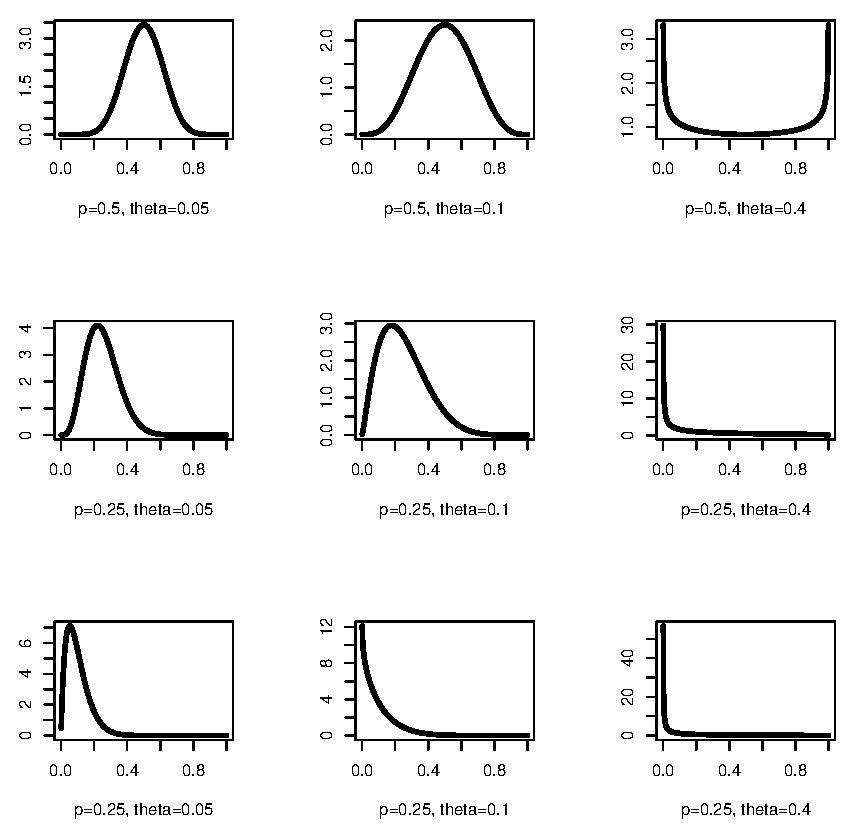
\includegraphics{beta-distribution.eps}}
\caption{Shapes of the Beta distribution for different choices of
  $\pi$ and $\theta$. In the figure captions ``p'' corresponds to $\pi$,
  and ``theta'' corresponds to $\theta$.}\label{fig:beta}
\end{figure}

\subsection*{The {\it Isotoma petraea} example}

If we put the data we've analyzed before into {\tt Hickory}, we get
the results shown in Table~\ref{table:james} $f$ is the
within-population inbreeding coefficient, $F_{is}$, $\theta^{(II)}$ is
the Bayesian analog of Weir and Cockerham's $\theta$,\footnote{This
  isn't quite true. If you're interested, ask me about it. If you're
  really interested, take a look at~\cite{Song-etal-2006}.}  and
$G_{st}^B$ is the Bayesian analog of Nei's $G_{st}$.

\begin{table}
\begin{center}
\begin{tabular}{cccc}
\hline\hline
           &             & \multicolumn{2}{c}{Credible Interval} \\
Parameter  & Mean (s.d.)     & 2.5\% & 97.5\% \\
\hline
$f$            & 0.52 (0.10) & 0.32 & 0.70 \\
$\theta^{(II)}$ & 0.19 (0.12) & 0.03 & 0.50 \\
$G_{st}^B$      & 0.10 (0.07) & 0.02 & 0.30 \\
\hline
\end{tabular}
\caption{Results from analyzing the {\it Isotoma petraea} data with
  {\tt Hickory}.}\label{table:james}
\end{center}
\end{table}

{\tt Hickory} allows you to select from three models when running the
data with codominant markers:

\begin{enumerate}

\item The {\tt full model} estimates both $f$ and $\theta^{(II)}$.

\item The {\tt f $=$ 0 model} constrains $f=0$ and estimates
  $\theta^{(II)}$. 

\item The {\tt theta $=$ 0 model} constrains $\theta^{(II)} = 0$ and
  estimates $f$.

\end{enumerate}

As a result, we can use DIC comparisons among the models to determine
whether we have evidence for inbreeding within populations ($f=0$ {\it
  versus} $f \ne 0$) or for genetic differentiation among populations
($\theta^{(II)}=0$ {\it versus} $\theta^{(II)} \ne 0$). If we do that with these
data we get the results shown in Table~\ref{table:dic}.\index{Deviance Information Criterion}

\begin{table}
\begin{center}
\begin{tabular}{cc}
\hline\hline
Model & DIC \\
\hline
Full             & 331.2 \\
$f=0$            & 355.4 \\
$\theta^{(II)}=0$ & 343.7 \\
\hline
\end{tabular}
\caption{DIC analysis of the {\it Isotoma petraea\/}
    data.}\label{table:dic}
\end{center}
\end{table}

The $f=0$ has a much larger DIC than the full model, a difference of
more than 20 units. Thus, we have strong evidence for inbreeding in
these populations of {\it Isotoma petraea}.\footnote{Much stronger
  than the evidence we had for inbreeding in the ABO blood group data,
  by the way.} The $\theta^{(II)} = 0$ model also has a DIC
substantially larger than the DIC for the full model, a difference of
more than 10 units. Thus, we also have good evidence for genetic
differentiation among these populations.\footnote{It's important to
  remember that this conclusion applies {\it only\/} to the locus that
  we analyzed. Strong differentiation at this locus need not imply
  that there is strong differentiation at other loci.}

If we ask {\tt Hickory} to keep log files of our analyses, we can also
compare the estimates of $f$ for the full and $\theta^{(II)}=0$
models. The posterior means are 0.52 and 0.55, respectively, so they
seem pretty similar. But we can do better than that. Since we have the
full posterior distribution for $f$ in both models, we can pick points
at random from each, take their difference, and construct a 95\%
credible interval. Doing that we find that the 95\% credible interval
for $f_{full} - f_{\theta^{(II)}=0}$ is (-0.29, 0.24), meaning we have
no evidence that the estimates are different. That may be a little
surprising, since we strong evidence that $\theta^{(II)} \ne 0$ in
these data, but it's also good news. It means that our estimate of
within-population inbreeding is not much affected by the amount of
differentiation among populations.\footnote{And when you say it that
  way, it sort of makes sense, doesn't it?} What may be more
surprising is that the estimates for $\theta^{(II)}$ with and without
inbreeding are also very similar: 0.19 {\it versus\/} 0.22,
respectively. Moreover, the 95\% credible interval for
$\theta^{(II)}_{full} - \theta^{(II)}_{f=0}$ is (-0.38, 0.33). Thus,
even though we have strong evidence that $f > 0$, our estimate of
$\theta^{(II)}$ is not strongly affected by what we think about $f$ in
these data.

\begin{table}
\begin{center}
\begin{tabular}{c|ccc}
\hline\hline
Method & $F_{is}$ & $F_{st}$ \\
\hline
Direct            & 0.14 & 0.21 & 0.32 \\
Nei               & 0.31 & 0.24 & 0.47 \\
Weir \& Cockerham & 0.54 & 0.04 & 0.56 \\
Bayesian          & 0.52 (0.32, 0.70) & 0.19 (0.03, 0.50) \\
\hline
\end{tabular}
\end{center}
\caption{Comparison of $F_{is}$ and $F_{st}$ estimates calculated in
  different ways.}\label{table:compare}
\end{table}

One more thing we can do is to look at the posterior distribution of
our parameter estimates and at the sample trace.\footnote{You may have
  discovered that you can do this in {\tt WinBUGS}
  too.}~(Figure~\ref{fig:james}). The result of an MCMC analysis, like
the ones here or the ones in {\tt WinBUGS}, is a large number of
individual points. We can either fit a distribution to those points
and display the results (the black lines in the figures), or we can
use a non-parametric, kernel density estimate (the blue lines in the
figures). The sample traces below show the values the chain took on at
each point in the sampling process, and you can see that the values
bounced around, which is good.

\begin{figure}
\resizebox{\textwidth}{!}{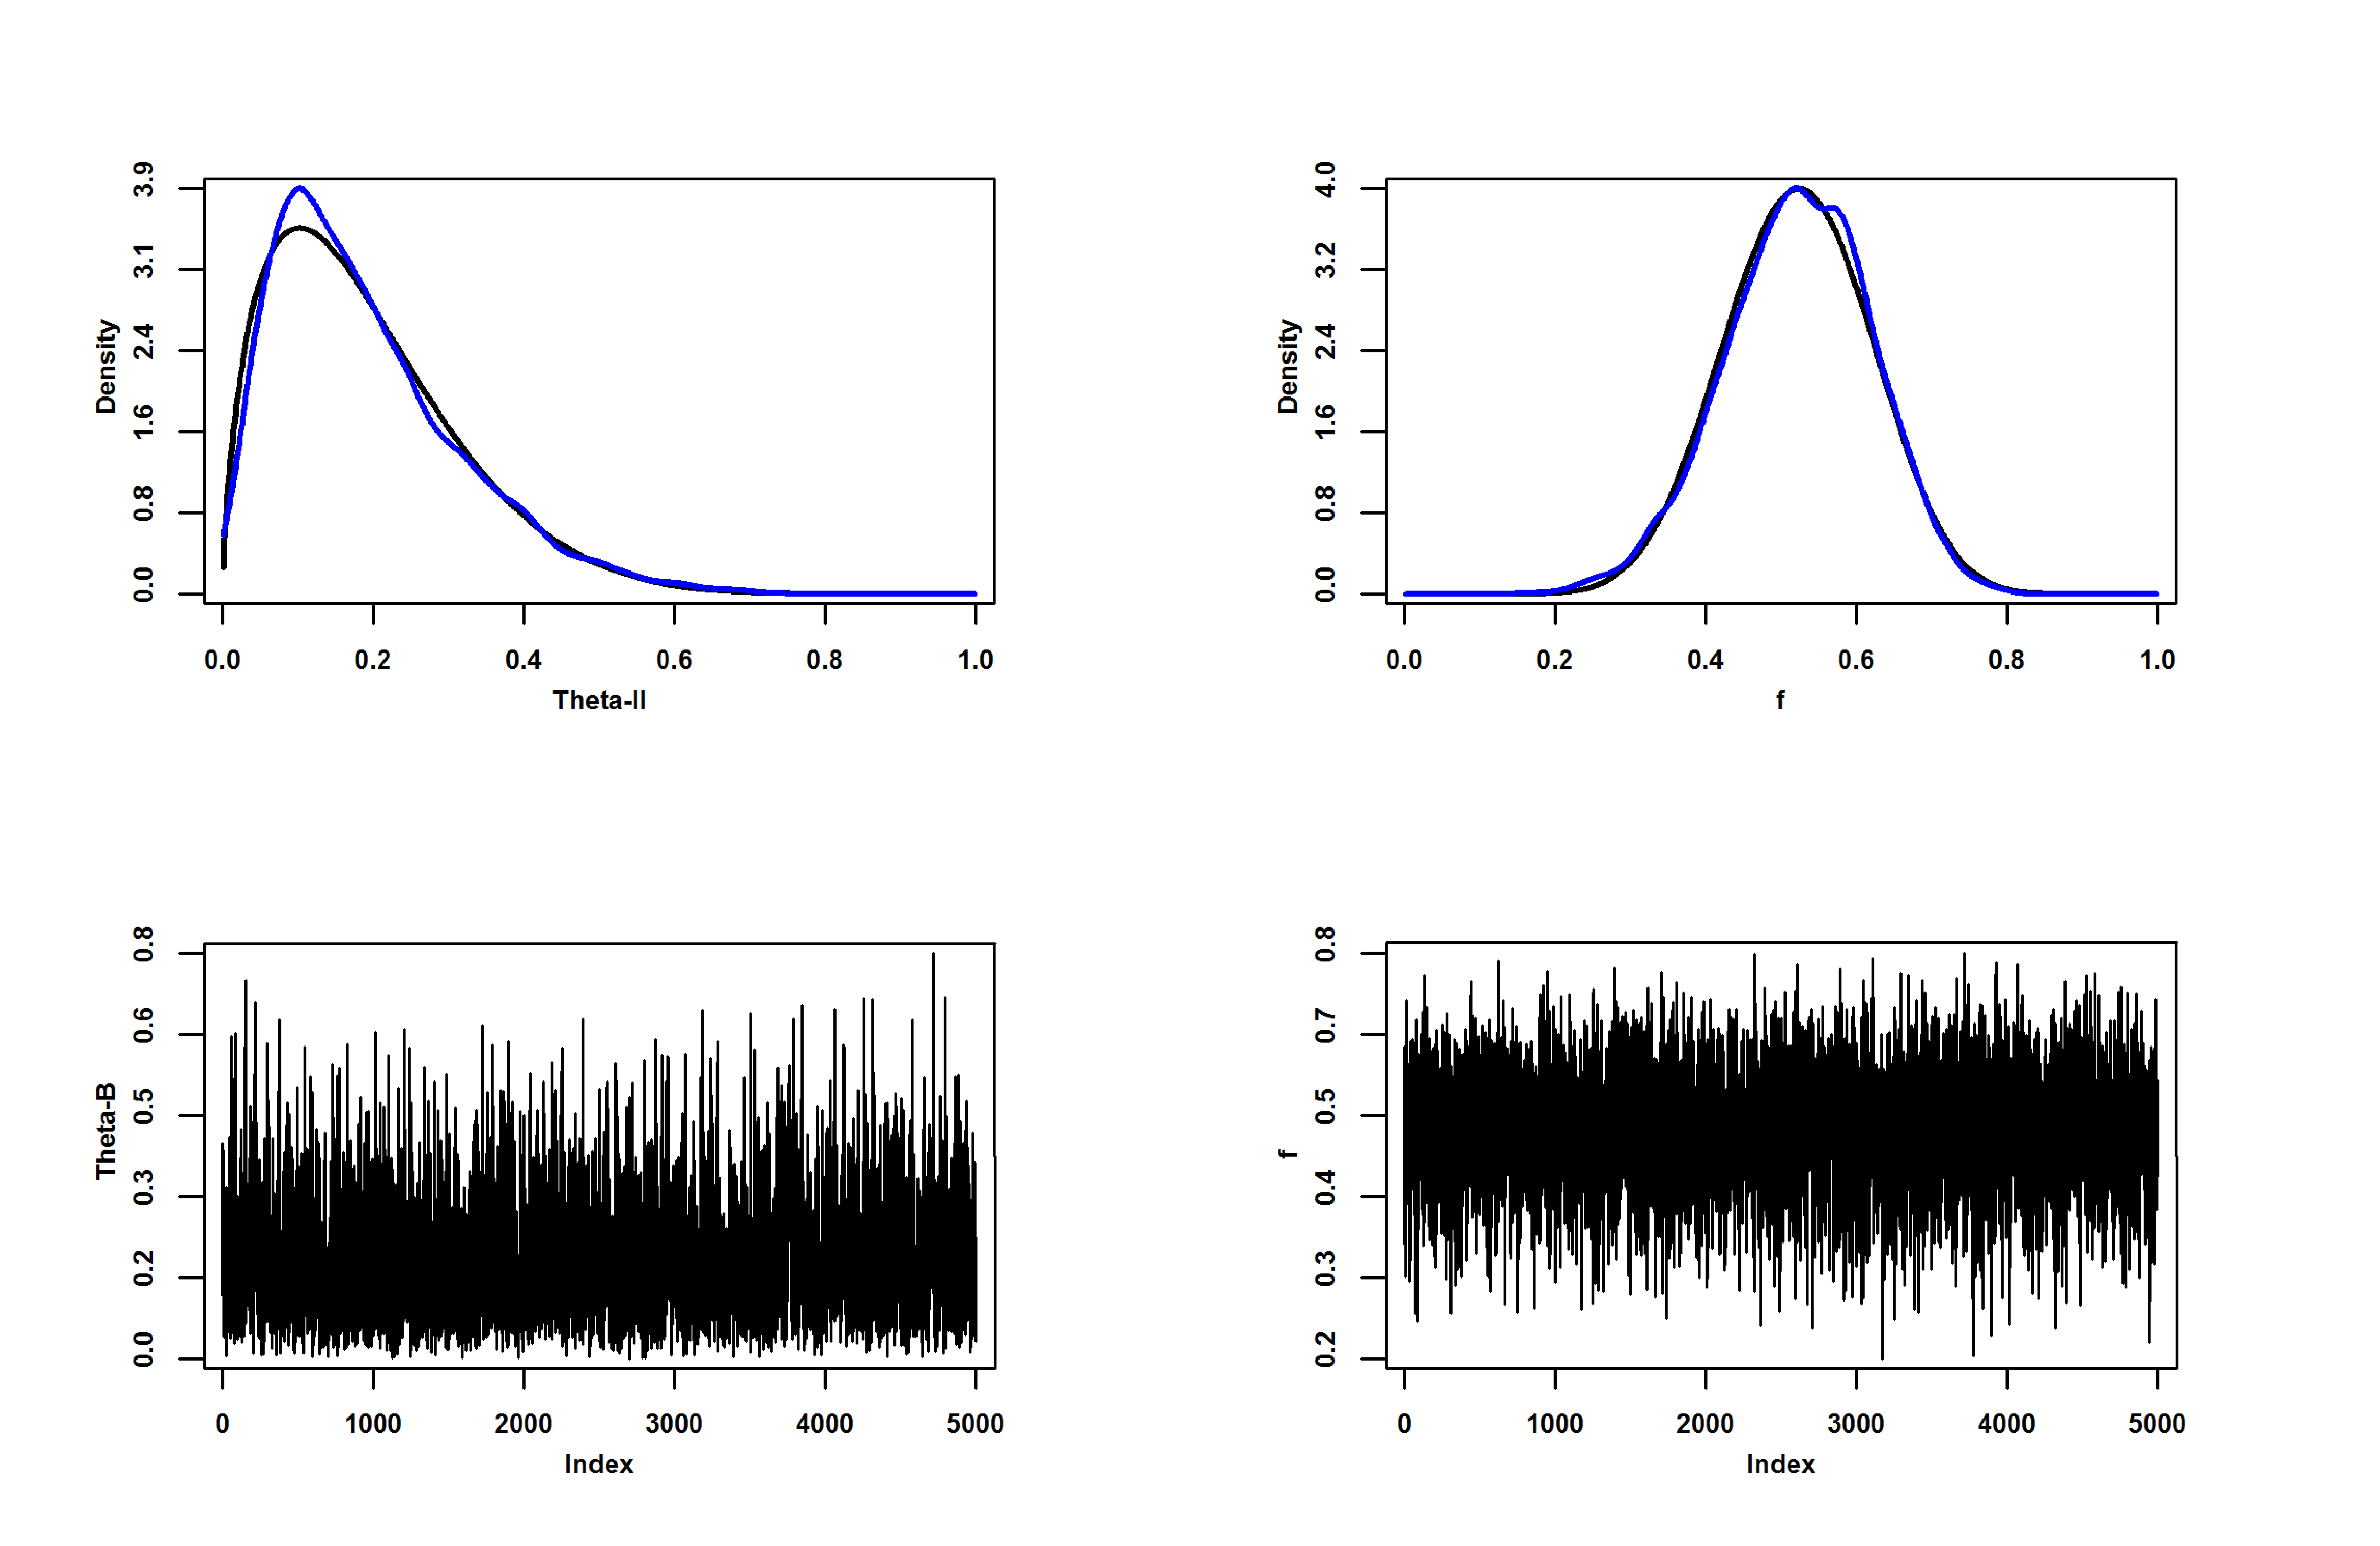
\includegraphics{james.eps}}
\caption{Posterior densities and traces for parameters of the full
  model applied to the {\it Isotoma petraea} data.}\label{fig:james}
\end{figure}

It's also useful to look back and think about the different ways
we've used the data from {\it Isotoma
  petraea}~(Table~\ref{table:compare}). Several things become apparent
from looking at this table:

\begin{itemize}

\item The direct calculation is very misleading. A population that
  has only one individual sampled carries as much weight in
  determining $F_{st}$ and $F_{is}$ as populations with samples of
  20-30 individuals.

\item By failing to account for genetic sampling, Nei's statistics
  significantly underestimate $F_{is}$, while Weir \& Cockerham's
  estimate is quite close to the Bayesian estimates.

\item It's not illustrated here, but when a reasonable number of loci
  are sampled, say more than 8-10, the Weir \& Cockerham estimates and
  the Bayesian estimates are quite similar. But the Bayesian estimates
  allow for more convenient comparisons of different estimates, and
  the credible intervals don't depend either on asymptotic
  approximations or on bootstrapping across a limited collection of
  loci. The Bayesian approach can also be extended more easily to
  complex situations.

\end{itemize}

